%description: Math 290 HW Template

%%%%% Beginning of preamble %%%%%

\documentclass[12pt]{article}  %What kind of document (article) and what size

%Packages to load which give you useful commands
\usepackage{subfig}
\usepackage{graphicx}
\usepackage{float}
\usepackage{hyperref}
\usepackage{amssymb, amsmath, amsthm}
\usepackage{listings}

%Sets the margins

\textwidth = 6.5 in
\textheight = 9 in
\oddsidemargin = 0.0 in
\evensidemargin = 0.0 in
\topmargin = 0.0 in
\headheight = 0.0 in
\headsep = 0.0 in
\parskip = 0.2in
\parindent = 0.0in

%defines a few theorem-type environments
% \newtheorem{theorem}{Theorem}
% \newtheorem{corollary}[theorem]{Corollary}
% \newtheorem{definition}{Definition}

\newtheorem{definition}{Definition}
\newtheorem{example}{Example}
\newtheorem{fact}{Fact}
\newtheorem{remark}{Remark}
\newtheorem{theorem}{Theorem}
\newtheorem{proposition}{Proposition}
\newtheorem{lemma}{Lemma}
\newtheorem{corollary}{Corollary}

\renewcommand{\labelenumi}{\arabic{enumi}.}
\renewcommand{\labelenumii}{\arabic{enumi}.\arabic{enumii}.}
\renewcommand{\labelenumiii}{\arabic{enumi}.\arabic{enumii}.\arabic{enumiii}.}
\renewcommand{\labelenumiv}{\arabic{enumi}.\arabic{enumii}.\arabic{enumiii}.\arabic{enumiv}.}
\newlength{\alginputwidth}
\newlength{\algboxwidth}
\newcommand{\alginput}[1]{\makebox[1.5cm][l]{ {\sc Input:}} \parbox[t]{\alginputwidth}{{\it #1}}}
\newcommand{\algoutput}[1]{\makebox[1.5cm][l]{ {\sc Output:}} \parbox[t]{\alginputwidth}{{\it #1}}}
\newcommand{\algtitle}[1]{\underline{Algorithm \ {\bf #1}} \vspace*{1mm}\\}

%%%%% End of preamble %%%%%







\begin{document}

\title{Senior Project (draft)\\
Lafayette College \\
Department of Mathematics
}

\author{
{Wah Loon Keng}\thanks{
Lafayette College,
Easton, PA 18042, USA.
kengw{\tt @}lafayette.edu.}
% \qquad
% {Benjamin H. Draves}\thanks{
% Lafayette College,
% Easton, PA 18042, USA.
% dravesb{\tt @}lafayette.edu.}
      % \affaddr{Department of Computer Science}\\
%       \affaddr{Lafayette College}\\
%       \affaddr{Easton, PA 18042, USA}\\
%       \email{gexia@cs.lafayette.edu}
}
% \date{}
\maketitle


\begin{abstract}
We conduct a survey study on machine learning, its mathematical foundations, general techniques, and the latest progress in both the academia and the industry. However, most machine learners  excel only at the task they are trained for - this is a huge limitation. Motivated by this, we study a new paradigm called the Never-Ending Language Learning (NELL)$^{\ref{NELL}}$ and its potentials to overcome the singular nature of machine learners. Lastly, we design and implement a system based on NELL to predict the stock market performance. This is driven by the abundance of data, and the complex, interacting, non-singular nature of the task that a machine learner has yet to match a human on.
\end{abstract}


\clearpage
\tableofcontents
\clearpage






\section{Introduction} \label{intro}

We have just entered the golden age of machine learning. The field has in fact been around for decades, born from artificial intelligence and pattern recognition. It wasn't until recently that we had the level of computational power and the abundance of data to apply it. 

The machine learners have accomplished some truly astonishing feats. They are systems that are trained with a copious amount of data, which allows them to surpass the performance level of human experts. Today, they are actively being researched and deployed by the biggest tech companies such as Google, IBM, Microsoft, Facebook. In fact, their major products are powered by machine learning - Google Adsense, IBM Watson, and Facebook's M - doing tasks such as ads suggestion, image recognition, medical diagnosis, and natural language processing.

Typically, machine learning is best suited for the tasks that cannot be solved precisely or efficiently by algorithms. Many of these are what humans excel at - image recognition, language processing, pattern deduction. These capabilities are so trivial to us, yet they are so difficult to mimic by traditional algorithmic approaches. The prime example of {\em ``a child can easily recognize a cat in a picture, but a super computer can't''} best illustrates the failure of the algorithmic methods. Machine learning comes in to save the day.

In a nutshell, one can think of a it as a machine that ``learns'' from the data. On the implementation level, it is an automated regression software that can construct an impressively accurate model. The machine takes in a training set - input data where each entry is labeled with the intended output, then trains on it and learns to recognize the pattern. After that, when fed with new unlabeled input, it gives some predicted output based on its training. However, just like a typical regression model, its scope is strictly bounded to its training set. For example, a machine that recognizes cats cannot recognize a fish without extra training. Moreover, an image recognizer cannot diagnose diseases. In this sense a machine learner's scope is {\bf singular}. We will address this issue later.

The mathematical foundations of machine learning is built atop regression theory and linear algebra. Next, we present the formalization of a problem in machine learning as well as the terminologies.








\subsection{Formalization}

The following formalization is standard in the literature, we reference Tom M. Mitchell's popular textbook {\em Machine Learning}$^{\ref{Mitchell}}$.


\begin{definition}
A computer program is said to {\bf \em learn} from experience $E$ with respect to some class of tasks $T$ and performance measure $P$, if its performance at tasks in $T$, as measured by $P$, improves with experience $E$.
\end{definition}

We will use the terms {\em training} and {\em learning} interchangeably. Next, we define a {\bf problem}.

\begin{definition}
A {\bf \em problem} is a triple $\{T, P, E\}$. The goal of a machine learner solving the problem is to output a learned target function $\hat{V}$ that approximates an ideal target function $V$. The target function maps from the vector of input features $b$ to the set of output $O$.
\end{definition}


The experience $E$ represents the input data. It is the set of points specifying the configurations of the instances of the problem. To use it for training, the data must be {\em labeled / classified} - every input data must have its output. This is needed for the performance measure $P$. In the context, it is understood that the data is always labeled.

Often the data set is split into three parts - the training set, validation set, and test set, for obvious statistical reasons. The first is used to weight-tuning (see below) that may yield multiple candidates, the second for validating and choosing the best candidate, and the last for testing against new input data and detecting overfitters. 


The feature vector $b$, output $O$, and the function representation for $\hat{V}$ are defined by the programmer as deemed suitable. In a simple regression model, $b$ is a list of chosen input features, $O$ is the set of predicted values. Typically the target function $\hat{V}$ will include a set of weights $W = \{w_i \ | \ i \in \{1,2,\cdots,n\}\}$ which are tuned during the learning. They serve as the ``memory'' of the machine to compute predicted output once it is trained.



Upon having an explicit representation, and given the training data, we can devise the learning mechanism. First, define an error term $\mathcal{E}$ between the training data and the actual machine output. Then, use the error term to devise an algorithm that tunes the weights iteratively to minimize the error. The algorithm terminates on meeting a minimum threshold error, that is when the machine can perform sufficiently good.

\begin{example}
We provide an explicit example with the checkers game:

{\bf The checkers learning problem:}
\begin{enumerate}
\item Task $T$: playing checkers
\item Performance measure $P$: percent of games won
\item Training experience $E$: games played against another computer
\end{enumerate}

Next we need to determine the representations of the available knowledge. For the input feature vector $b$, we can choose a few board states, for instance, 
$$b = \langle x_1, x_2, x_3, x_4 \rangle$$
where the $x_i$'s are respectively the numbers of black pieces, black kings, red pieces and red kings on the board. We can choose a simple linear combination as our target function,
$$\hat{V}(b) = w_0 + w_1 x_1 + w_2 x_2 + w_3 x_3 + w_4 x_4$$
where $w_i$'s are the weights to be tuned during the training. Our output set $O$ is the list of moves at each game step given the features $x_i$'s at the time. We can define a bijection between the output range of $\hat{V}(b)$ and the $O$, but we will exclude it here.

Once we have a representation, devise a learning mechanism for training. Suppose now we have a set of positive (games won) training examples $\{\langle b, V_{train}(b) \rangle\}$. Define the error term using simple sum of squares $$\mathcal{E} = \sum_{\langle b, V_{train}(b) \rangle \in \ {\rm training\ examples}} (V_{train}(b) - \hat{V}_{train}(b))^2$$

Then, using this, devise an algorithm $A$ for training / weight-tuning. The error term above, when differentiated, yields gradient term of $\sim(V_{train}(b) - \hat{V}_{train}(b))$. One can imagine training as nodging a point closer to its true value, and the gradient gives the direction to nodge towards. This gives us a simple LMS algorithm for minimizing $\mathcal{E}$ using that gradient term:


\algtitle{LMS weight-tuning (learning) algorithm}
Initialize the weights $w_i$'s to random values. For each training example $\langle b, V_{train}(b) \rangle$:
\begin{enumerate}
	\item Use the current weights to compute $\hat{V}(b)$
	\item For each weight $w_i$, update it by $$w_i \leftarrow w_i + \eta \ (V_{train}(b) - \hat{V}_{train}(b)) \ x_i$$
\end{enumerate}

where $\eta$ is the parameter that moderates the stepsize. The algorithm terminates when $w_i$'s stop changing, i.e. when the error becomes sufficiently small (zero).

\end{example}

One can quickly see that the example machine learner above is just a simple regressor. Obviously this toy model will not be a good checker player. Nevertheless, given a huge training data, if we choose the right knowledge representation, feature vector $b$, target function $\hat{V}$, error term $\mathcal{E}$, and the learning algorithm, the resultant machine can perform very well. 

To suit a different type of problem, we can employ a different {\bf representation} - which we define to be the set $\{T, P, E, b, O\}$, as illustrated in Table \ref{rep}.



\begin{table}[ht]
\begin{center}
\begin{tabular}{ | l | l | l || l | l | }

\hline
$T$ & $P$ & $E$ & $b$ & $O$ \\
\hline \hline
image recognition & correct labeling & labeled images & array of pixels & label of objects \\
\hline
driving a car & successful trip & test drives & traffic condition & wheel, pedals  \\
\hline
text translation & correct translations & pretranslated texts & semantics & translated text \\
\hline
ads suggestion & ads click rate & ads metadata & user profile & ads displayed \\
\hline
\end{tabular}
\caption{Different representations for various problems.}
\label{rep}
\end{center}
\end{table}



Moreover, we can employ different {\bf learning mechanisms} - which we define as the set of target function and learning algorithm, $\{\hat{V}, A\}$. This gives rise to the different techniques, or types, of machine learners such as the Neural Nets, Support Vector Machines, Deep Learning and etc. We will investigate the popular types in the next section.

A huge variety of machine learners today are being used for different purposes - most of the leading tech companies tweak and design their own. They may have very different {\bf representations} and {\bf learning mechanisms}, but the overall idea is still the same - gather labeled data, define the representations and learning algorithms, and train. The entire process is very modular, and the resultant machines are {\bf stagnant} - the machine no longer improve once training is done; and {\bf singular} - they can only function very narrowly only on the tasks they are trained for. For our discussions, we call this the {\bf stagnant \& singular paradigm}. In fact, this paradigm can readily be observed across most of the popular machine learners today. This will serve as the primary motivation of our work.









% \subsection{Popular Techniques}

Before getting to the discussion on the paradigm, we take a quick look at the most common and powerful machine learners. These are derived from the same {\bf stagnant \& singular paradigm} by varying the {\bf representations} and {\bf learning mechanisms}.



% \section{Decision Tree}

% Decision tree is an old method stemmed from artificial intelligence, used for hypothesis-searching and inductive reference. It uses a {\em tree representation}, where each node is a feature variable, and each edge is a value the feature takes on. The leaf nodes are the classification (output) values. Every path from the root to the leaf represents an instance of the feature $b$ and its output $o$. Moreover, different paths can be combined with logical $OR$ and $AND$ to yield a more general hypothesis space.

% For the {\em learning mechanism}, a common method is to use the entropy measure and entropy gain while branching on each node (making a decision) while descending the tree. Suppose the data has $c$ classifications (e.g. $c=2$ for binary classifiers), the entropy is defined as $$Entropy(D) = \sum_{i=1}^{c} -p_i \ log_2 \ p_i$$ where $D$ is the data, $p_i$ is the proportion of samples of class $i$ in $D$. This allows us to judge the performance $P$ and search for the target function $\hat{V}$ by using the entropy gain for each feature $b$, $$Gain(D,b) = Entropy(D) - \sum_{v\in Values(b)} \frac{|D_v|}{D} Entropy(D_v)$$ where $D_v$ is the subset of D whose feature vector assumes the values equals to $v$.

% Each path in the tree is a candidate hypothesis (collection of contributing features) to consider. Given the multitude of paths in the tree, the algorithm will end up with a set valid and consistent hypotheses. To resolve this, we simply use the {\bf Occam's razor} - choose the simplest hypothesis that fits the data. This will also prevent the initial overfitting.



\section{Artificial Neural Network (ANN)}

Often called just the ``neural net'', ANN was inspired by the biological system of neurons in the brain (note that it is inconsistent with the biological version). This is one of the earliest techniques, and has improved over the decades; the first practical usage was in the 80's, and today it is one of the most popular with countless variations. Here, we will describe the original and the most common designs.

Neural network is a practical method for learning examples that are real-valued, discretized, and multi-dimensional. It is so general that it has been applied successfully to image recognition, pattern-identification, robotics, speech and many more. Its popularity is primarily due to its power to learn accurately and its simplicity.

An ANN is a directed graph whose nodes are the feature variables, and edges are the weights. It is ordered into layers of nodes that are adjacently bipartite, i.e. every node in each layer connects (directionally) to all the nodes in the next layer. The first is called the {\em input layer}, the last the {\em output layer}, and the rest in between the {\em hidden layers}. A node is also called a {\em unit}, and those in the {\em hidden layers} are called {\em hidden units.}

The {\em input layer} corresponds to the feature vector $b$ - each unit takes the value for each feature variable. Similarly the output layer corresponds to the output $o$. Each iteration of training involves a series of computation from the input, through the hidden layers, to the output. Across the net, the outputs become the inputs for the next layer.

Suppose we have at layer $i$ indexed nodes $x_{i,1}, x_{i,2}, \cdots, x_{i,p}$ bipartite to nodes $x_{i+1,1}, x_{i+1,2}, \cdots, x_{i+1,q}$ at layer $i+1$. We can simply represent as the edges with their weights with subscript indicating the connection. For example, the first node $x_{i,1}$ connects to all the edges in the next layer via $w_{i,1,1}, w_{i,1,2}, \cdots, w_{i,1,q}$.

Then, we can define the function for mapping input values at $x_{i,1}, x_{i,2}, \cdots, x_{i,p}$ to an output value at $x_{i+1,j}$, i.e. we can define a target function for an output node $x_{i+1,j}$ $$\hat{V}_{i+1,j} : \{ w_{i,1,j}, w_{i,2,j}, \cdots, w_{i,p,j} \} \times \{ x_{i,1}, x_{i,2}, \cdots, x_{i,p} \} \mapsto x_{i+1,j}$$

Typically, an inner product is sufficient to yield a good ANN. For this we have the form $$\hat{V}_{i+1,j} = \langle  w_{i,1,j}, \cdots, w_{i,p,j}  \rangle \cdot \langle  x_{i,1}, \cdots, x_{i,p}  \rangle = w_{i,1,j}x_{i,1} + \cdots + w_{i,p,j}x_{i,p}$$

\begin{figure}
\centering
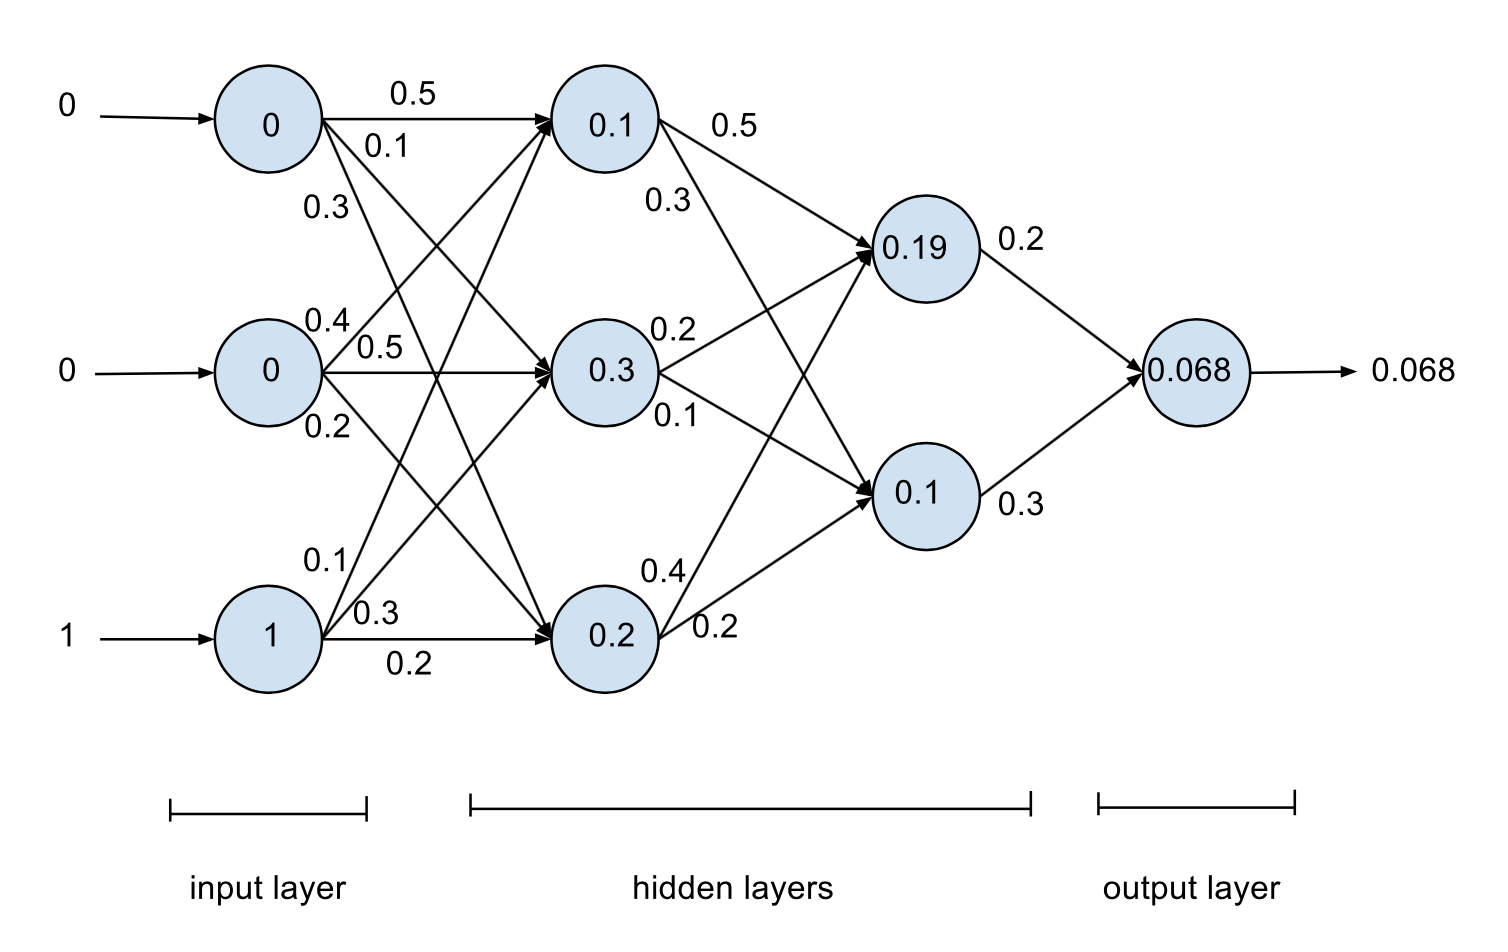
\includegraphics[scale=0.5]{images/ANN.png}\\
\caption{An ANN with 3 input units, 2 hidden layers each with 3 and 2 hidden units, and 1 output unit. The target function is the dot product between the incident values from the previous layer and their edge weights.}\label{ANN-fig}
\end{figure}

An explicit example is provided in Figure \ref{ANN-fig}. The feature vector input is $b = \langle 0,0,1 \rangle$; the value $$x_{2,1} = \hat{V}_{2,1} = w_{1,1,1}x_{1,1} + w_{1,2,1}x_{1,2} + w_{1,3,1}x_{1,3} = 0.5 \cdot 0 + 0.4 \cdot 0 + 0.1 \cdot 1 = 0.1$$

If we wish, we can define the target function $\hat{V} : b \mapsto o$ for the entire ANN by taking the ordered composition of the sub-target functions defined above, but this is cumbersome. Often the graph representation is used.

We can create variations of ANN by tweaking the target function $\hat{V}$, the error term $\mathcal{E}$, and the training algorithm $A$. Moreover, we can change the graph structures by adding more hierarchies (convolutional, deep learning) or {\em backedges} to create cycles (recurrent neural network RNN).

With data $\{\langle b, V(b) \rangle\}$, the training goes as usual. A single iteration of training starts from the input layer and ends at the output layer. The error term is then used with the tuning algorithm $A$ to tune the edge weights, i.e. use the errors to update the weights. Reiterate the process until the output error is smaller than a threshold. Unsurprisingly, training a large neural net can take up to months, but the results can be very impressive. Below, we describe some of the most powerful versions that have recently made the news.





\subsection{ANN with Perceptrons}

Given the general design above, we can simplify our notations to aid discussions. Focusing on a subnetwork, look at a single output unit $o$ with incoming inputs $x_1, x_2, \cdots, x_k$ and weights $w_1, w_2, \cdots, w_k$, the target function for a perceptron unit is
\[
o(x_1, \cdots, x_k) =
\begin{cases}
1 &\text{if } w_0 + w_1 x_1 + w_2 x_2 + \cdots + w_k x_k > 0\\
-1 &\text{otherwise }
\end{cases}
\]

Concisely, we write $$o(\vec{x}) = sign(\vec{w} \cdot \vec{x})$$

The training rule for the algorithm is a simple update, $$w_i \leftarrow w_i + \eta(t-o)x_i$$ where $\eta$ is the stepsize moderation called the {\em learning rate}, $t$ is the target output value, $o$ the actual perceptron output, $x_i$ the input node value.




\subsection{ANN with Gradient Descent}

The gradient descent can be seen as a refinement to the perceptron. Its target function is $$o(\vec{x}) = \vec{w} \cdot \vec{x}$$

The unit is called a {\em linear unit} for an obvious reason. The error term is defined as $$\mathcal{E}(\vec{w}) = \frac{1}{2} \sum_{d \in D} (t_d - o_d)^2$$ where $D$ is the data, $t_d$ is the target output value, $o_d$ the unit output for a data point $d$. This will guide the weight-tuning rule for the algorithm, which also gives its name.

Given the formalism, we can equivalently view as a vector space. Our task then is to find the set of weights that yields the right target function. Minimizing the error term is then equivalent to minimizing the error surface in the vector space. We know this is done by stepping in the direction of the steepest descent along the error surface, which is simply the gradient of the error term $$\nabla \mathcal{E}(\vec{w}) =\ \langle  \frac{\partial \mathcal{E}}{\partial w_0}, \frac{\partial \mathcal{E}}{\partial w_1}, \cdots, \frac{\partial \mathcal{E}}{\partial w_k}  \rangle$$

Then, the tuning rule is simply $$\vec{w} \leftarrow \vec{w} - \eta \nabla \mathcal{E}(\vec{w})$$ where $\eta$ is the learning rate. When written in component form we get $$w_i \leftarrow w_i - \Delta w_i = w_i - \eta \frac{\partial \mathcal{E}}{\partial w_i}$$


\algtitle{Gradient-Descent(Data, $\eta$)}
Each training example $d \in Data$ is of the form $d = \langle \vec{x}, t \rangle$, where $\vec{x}$ is the input vector, $t$ the target output value, $\eta$ the learning rate. Note that the partials are found using discretized iterations at step 2.2.2.

\begin{enumerate}
	\item Initialize the weights $w_i$'s to small random values.
	\item Until termination condition (defined separately), do
		\begin{enumerate}
			\item Initialize each $\Delta w_i$ to 0
			\item For each $\langle \vec{x}, t \rangle \in Data$, do 
			\begin{enumerate}
				\item Input $\vec{x}$ and computer output $o$
				\item For each unit weight $w_i$, do $$\Delta w_i \leftarrow w_i + \eta(t-o)x_i$$
			\end{enumerate}
			\item For each linear unit weight $w_i$, do $$w_i \leftarrow w_i + \Delta w_i$$
		\end{enumerate}
\end{enumerate}





\subsection{ANN with Backpropagation}

The invention of {\em Backpropagation} by Geoffrey Hinton and Yann LeCun reinvigorated ANN after its loss of popularity due to practical limitations. First, we improve the target function by using a sigmoid (logistic) function, yielding a {\em sigmoid unit} $$o = \sigma (\vec{w} \cdot \vec{x})$$ where $$\sigma(y) = \frac{1}{1+e^{-y}}$$ It has some very nice properties. The function maps the entire real domain into $(0,1)$ like a ``squeezing function'' with the outlier points getting pushed to the narrow ends of the interval; it increases monotonically; it is smooth with a convenient derivative $\sigma'(y) = \sigma(y) (1 - \sigma(y))$, which is computationally cheap.

Next, {\em Backpropagation} can efficiently train a large multilayer network. We can directly generalize the error term as the sum over all nodes at a layer, $$\mathcal{E}(\vec{w}) = \frac{1}{2} \sum_{d \in D} \sum_{k \in outputs} (t_{d,k} - o_{d,k})^2$$

The following algorithm constructs an ANN that uses {\em Backpropagation} with the number of units as parameters.


\algtitle{Backpropagation(Data, $\eta$, $n_{in}$, $n_{out}$, $n_{hidden}$)}
Each training example $d \in Data$ is of the form $d = \langle \vec{x}, t \rangle$, where $\vec{x}$ is the input vector, $t$ the target output value, $\eta$ the learning rate. $n_{in}$, $n_{out}$, $n_{hidden}$ are respectively the numbers of units in the input, hidden and output layers. Double indices are ordered as {\em from, to}. Note that the partials are found using discretized iterations at step 3.1.2.

\begin{enumerate}
	\item Create a feed-forward network with $n_{in}$ inputs, $n_{hidden}$ hidden units, and $n_{out}$ output units.
	\item Initialize all weights to small random values.
	\item Until termination condition (defined separately), do
		\begin{enumerate}
			\item For each $\langle \vec{x}, t \rangle \in Data$, do:
			\begin{enumerate}
				\item (Propagate the input through the network) Input $\vec{x}$ and computer output $o$ for every unit
				\item (Propagate the errors backward through the network) For each output unit $o_k$, compute its error term $\delta_k$ by $$\delta_k \leftarrow o_k(1-o_k)(t_k-o_k)$$
				\item For each hidden unit $h$, compute its error term $\delta_h$ by $$\delta_h \leftarrow o_h(1-o_h)\sum_{k \in outputs}w_{hk}\delta_{k}$$
				\item Update each weight $w_{ij}$ by $$w_{ij} \leftarrow w_{ij} + \Delta w_{ij}$$ where $$\Delta w_{ij} = \eta \ \delta_j \ x_{ij}$$
			\end{enumerate}
		\end{enumerate}
\end{enumerate}


There are obvious caveats to {\em Backpropagation}, namely convergence and local minima. The former can be resolved by added heuristics in the externally-defined termination condition; the latter can be overcome by updating the algorithm with {\em stochastic gradient descent} instead. Fortunately for most practical purposes, these limitations can safely be ignored.

This ANN is in fact so powerful that it can represent every Boolean function, approximate any continuous functions, as well as arbitrary functions. The {\em Universal Approximation Theorem}$^{\ref{Cybenko}}$ states that a feedforward ANN with three layers of units can achieve this generality.

Since its invention in the 80's it has become the primary method for ANN. Indeed thus far in this paper, {\em Backpropagation} is the most powerful machine learner, until the recent rise of the more powerful {\em Deep Learning.}



\section{Deep Neural Network (DNN)}

The most popular and powerful machine learning technique today is undoubtedly deep learning, given the impressive accomplishments by \emph{IBM Watson, Facebook M}, and \emph{Google Tensorflow} this year. The theoretical foundation has been around for decades, but it wasn't until now that we had the level of computational power and abundance of data to apply it.

Deep learning is implemented as a Deep Neural Network (DNN), which is itself a neural net. The term \emph{deep} stands for the depth of the hidden layers of DNN. Whereas most ordinary ANNs are ``shallow'' with less than 3 hidden layers, DNNs are ``deeper'' with many (usually over 3) hidden layers. It turns out that having more hidden layers can make a neural net immensely more powerful that it can represent a larger class of functions.


\begin{figure}[ht]
\centering
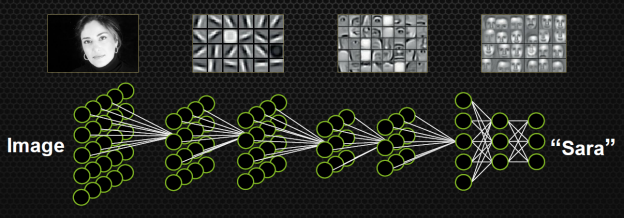
\includegraphics[scale=0.9]{images/DNN.png}\\
\caption{DNN that mimics the hierarchical structure of the brain. Going from left (input) to right, features get generalized from the specifics into more generic and abstract representations. At the top level (rightmost),  \href{http://devblogs.nvidia.com/parallelforall/accelerate-machine-learning-cudnn-deep-neural-network-library/}{\tt Image from NVIDIA.}}\label{DNN-fig}
\end{figure}


Having more hidden layers allows DNNs to progressively generalize features and abstractions. Going from the first to the last hidden layer, a DNN can capture features that are decreasingly specific and increasingly generic. For instance in face recognition, a DNN may capture the specific shades, then the eyes, nose, mouth features, then the shape, and finally a more invariant representation of the face of a person, say Sara in Figure \ref{DNN-fig}. It is the top level generalization that allows it to recognize a person's face regardless of the local variations, such as the head's orientation, the lighting, and the facial expression. In this aspect, DNNs are more ``brain-like'' than other machine learners, as we shall discuss more in depth later.


Whereas ANNs are \emph{supervised} (requires the training data to be labeled), There are two types of learning for DNNs, both of which are not supervised. \emph{Semi-supervised learning} is where unlabeled training data is drawn from the same prior distribution as the labeled training data; \emph{self-taught learning} does not have that requirement.

Next, we look at an \emph{autoencoder} - a basic but fundamental component of a DNN.

\subsection{Autoencoder}

The autoencoder is a neural net that learns the structure from an unlabeled data set. It has one hidden layer; the non-output layers (the first two) each has an extra \emph{bias} neuron that accepts no input and constantly outputs 1. Given an unlabeled data set of $n$ points, subscripted with $u$, $\{x^{(1)}_u, x^{(2)}_u, \cdots, x^{(n)}_u \}$, the autoencoder sets the outputs $y^{(i)} = x^{(i)}_u$, and train on the data $\{(x^{(1)}_u, y^{(1)}), \cdots, (x^{(n)}_u, y^{(n)}) \}$ as usual. Since the outputs are set to the input, we can view the autoencoder as a neural net that learns the identity function, and its tuned weights would uncover the structure in the data.


\begin{figure}[ht]
\centering
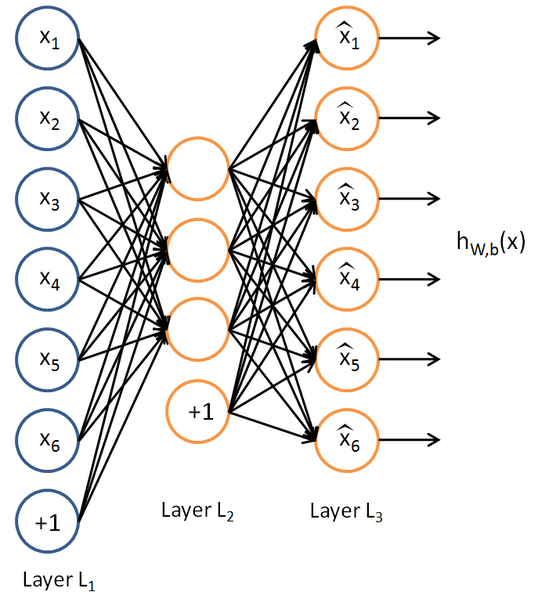
\includegraphics[scale=0.4]{images/autoencoder.png}\\
\caption{An autoencoder. The units with $+1$ are the bias units. The output units $\sf{\hat{x}_i}$ will try to converge to $x_i$, as autoencoder mimics an identity function. \href{http://deeplearning.stanford.edu/wiki/index.php/File:Autoencoder636.png}{\tt Image from UFLDL.}}\label{autoencoder-fig}
\end{figure}


We now introduce the tensorial notation used for DNNs.


\begin{table}[ht]
\begin{center}
\begin{tabular}{ | l | p{10cm} | }

\hline
$Symbol$ & $Meaning$ \\
\hline \hline
$x$ & The input features, $x \in \mathcal{R}^n$. \\
\hline
$y$ & The target values (vector), $y = x$ for autoencoder. \\
\hline
$(x^{(i)}, y^{(i)})$ & The $i^{th}$ training example. For autoencoders, $y^{(i)} = x^{(i)}$. \\
\hline
$L_l$ & The $l^{th}$ layer of the net. \\
\hline
$b^{(l)}_i$ & The bias unit at layer $l$ that points to unit $i$ in layer $l+1$ (think of it as the edge); outputs 1. \\
\hline
$W^{(l)}_{ji}$ & The weight going out from the $i^{th}$ node in layer $k$ to the $j^{th}$ node in layer $k+1$. Note the ordering of the indices, which is different from the previous sections. \\
\hline
$z^{l+1} = W^{(l)} a^{(l)} + b^{(l)}$ & The outputs of all unit from layer $l$, in compact tensorial form. Note that $a^{(1)} = x$. \\
\hline
$f(\cdot)$ & The activation function that transforms the input $z$ at each node into the activation $a = f(z)$. Applies element-wise to a tensor. Typically, we use a sigmoid function $f(z) = 1/(1+e^{-z})$. \\
\hline
$a^{(l)}$ & Activation, i.e. the transformed outputs of all units at layer. $a^{(l)} = f(z^{(l)})$. \\
\hline
$h_{W,b}(x) = a^{(3)} = f(z^{(3)})$ & The hypothesis of an autoencoder, given input features $x$, parametrized by the edge weights in the tensors $W, b$. \\
\hline
\end{tabular}
\caption{Tensorial notation for DNNs.}
\label{tensor-note}
\end{center}
\end{table}




\subsection{Hybrid Method}

One of the biggest hurdles to machine learing is the scarcity of labeled data. Every data point has to be manually labeled by humans - not every picture of a cat on the web is already tagged with ``cat''. Therefore, despite having a large trove of data today, most of it is unlabeled and thus remains unusable by supervised machine learners. 

The problem necessitates new approaches to make use of the unlabeled data - self-taught learning and semi-supervised learning as mentioned in the section on Autoencoders. However, a machine trained solely by these methods only learns the structure of the data, and cannot be very useful as its output approximates its input - it cannot be used as a general predictor.

Fortunately, we can do better by utilizing both the unlabeled and labeled data sets via a hybrid approach. First, we train the autoencoder to ``memorize'' the structure of the unlabeled data - this is called \emph{pretraining}. Then, we replace its output layer with a supervised ANN, and train the new network on the labeled data - this is called \emph{fine-tuning}. The result can have a far greater representational power. This is the basis of a DNN, and is illustrated in Figure \ref{sparseAE-fig}, \ref{LogisClass-fig} and \ref{combinedAE-fig}.



\begin{figure}[ht]
\centering
\begin{minipage}{.45\linewidth}
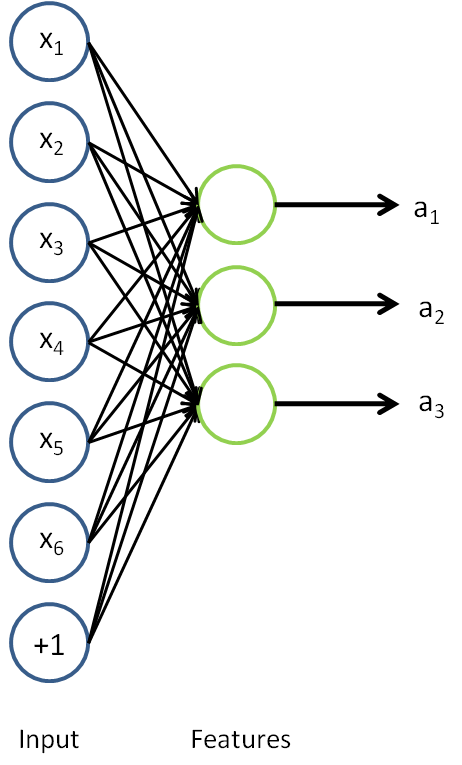
\includegraphics[scale=0.6]{images/SparseAE.png}\\
\caption{Self-taught learning: Pretraining Sparse Autoencoder - simply remove the third layer from the Autoencoder after training. \href{http://deeplearning.stanford.edu/wiki/index.php/Self-Taught_Learning_to_Deep_Networks}{\tt Image from UFLDL.}}\label{sparseAE-fig}
\end{minipage}
\hspace{.05\linewidth}
\begin{minipage}{.45\linewidth}
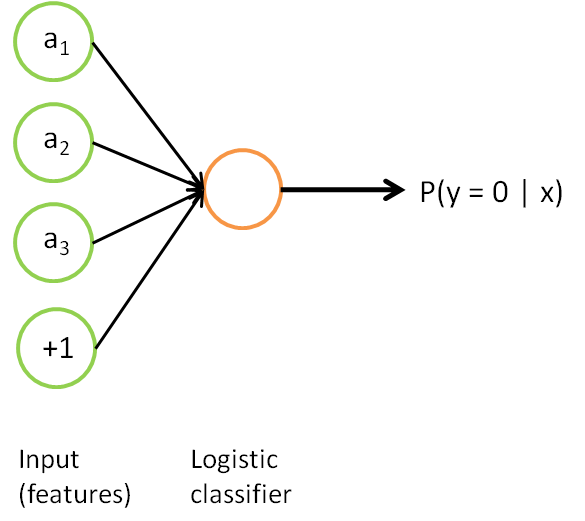
\includegraphics[scale=0.7]{images/Logistic_Classifier.png}\\
\caption{Supervised learning: Training Logistic Classifier (an ANN) using the activation units from the Sparse Autoencoder plus a bias unit. \href{http://deeplearning.stanford.edu/wiki/index.php/Self-Taught_Learning_to_Deep_Networks}{\tt Image from UFLDL.}}\label{LogisClass-fig}
\end{minipage}

\end{figure}


\begin{figure}[ht]
\centering
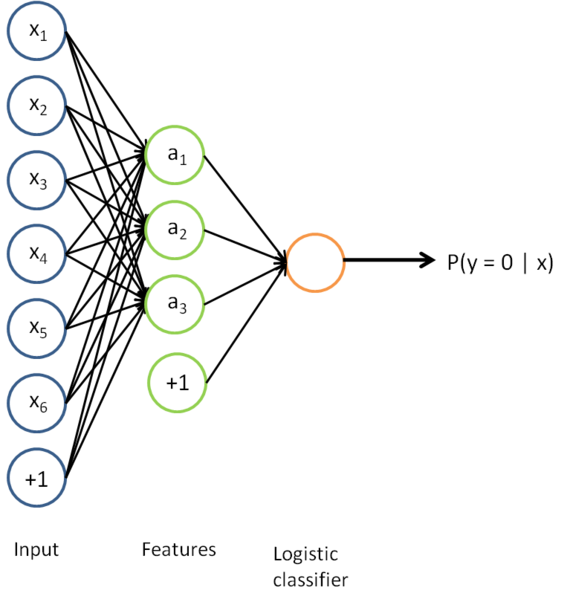
\includegraphics[scale=0.8]{images/CombinedAE.png}\\
\caption{Semi-supervised learning as the basis for deep-learning: The network obtained by combining the Sparse Autoencoder from pretraining and the logistic classifier from supervised training. \href{http://deeplearning.stanford.edu/wiki/index.php/Self-Taught_Learning_to_Deep_Networks}{\tt Image from UFLDL.}}\label{combinedAE-fig}
\end{figure}


The intuition is that \emph{pretraining} ``coarse-tunes'' the hidden layers into a guided configuration (of edge weights), which gives a better headstart than random weight initialization for training (\emph{fine-tuning}) on the labeled data set. As mentioned, this requires a large set of unlabeled training data. On top of that, we must have a comparably large set of labeled training data to use \emph{fine-tuning}. This hybrid method will significantly improve the performance of the network, and is key to the tremendous power of DNNs.






\subsection{Stacked Autoencoders}

Before we present a sample construction for a deep network with more hidden layers, two design features are crucial to making DNNs powerful and practical:

\begin{enumerate}
	\item The activation function $f(\cdot)$ must be non-linear. Otherwise, when composing the functions over the layers, the linear composition of linear functions is also linear, and thus would result is a far more restrictive representational power. Commonly the non-linear activation function of choice is the sigmoid function.
	\item ``Compactness'' can be achieved in the sense that $k$ hidden layers can represent what $k-1$ layers cannot unless the latter has exponentially more hidden units. Whereas to increase the representational power by adding a hidden layer, the number of units only grows polynomially. The deeper the network, the more powerful it is.
\end{enumerate}


Having more hidden layers also pose the following problems.

\begin{enumerate}
	\item \emph{Diffusion} occurs, in which the error adjustment during backpropagation with gradient descent diminishes across layers. This makes it harder for the front layers closer to the input to converge.
	\item A much larger amount of data is needed for training, and in some applications this is unfeasible.
	\item The functions approximated by the deeper network is highly non-convex, and therefore may converge to some bad local optima.
\end{enumerate}

The solutions to these are

\begin{enumerate}
	\item Greedy layer-wise training: train the network with $l$ layers, then add another hidden layer and retrain the network with $l+1$ layers.
	\item Utilize the abundant unlabeled data via \emph{pretraining}.
	\item After pretraining, the starting point is better, and \emph{fine-tuning} will often lead to a good local optima in practice.
\end{enumerate}


Generalizing from the previous construction, we now look at the \emph{Stacked Autoencoders}. The extension is straightforward. Below, we use the greedy layer-wise training on the autoencoder - train the network with $l$ layers, then stack another autoencoder on top and retrain the network with $l+1$ layers, therefore the name \emph{stacked autoencoder}.

Formally, a \emph{stacked autoencoder} is network of multiple layers of autoencoders. Each autoencoder (of 3 layers in total) at layer $l$ is trained on unlabeled data, then stripped of its output layer. The output from its hidden layer is then used as the input layer of the next added autoencoder at layer $l+1$ (thus adding a hidden and an output layer with the proper bias units). This process repeats up until we have the desired number of hidden layers. The training at layer $l$ for the autoencoder can be done locally while freezing the parameters of the other layers, which the input is injected and propagated to it from the first input layer of the network.

The activation units at layer $l$ is written in the tensorial notation as 
$$a^{(l)} = f(z^{(l)})$$
$$z^{(l+1)} = W^{(l)}a^{(l)} + b^{(l)}$$

Finally, when the greedy layer-wise pretraining using the unlabeled data is complete, a classifier (logistic, softmax, etc.) is added to the end of the network. We can now perform \emph{fine-tuning} – supervised training using the labeled data. The weights of the other layers shall now be allowed to change, as the entire network is being tuned. Backpropagation with gradient descent can be a good method for fine-tuning.

We give explicit illustrations of a deep network, which is a stacked autoencoder with 2 hidden layers, in Figure \ref{deep1}, \ref{deep2}, \ref{deep3}, \ref{deep4} that are easier to grasp visually.



\begin{figure}[H]
\centering
\begin{minipage}{.45\linewidth}
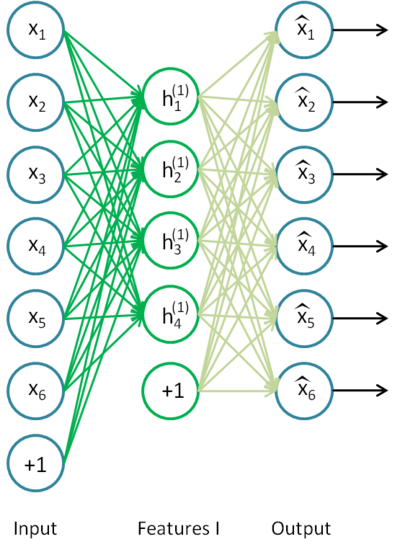
\includegraphics[scale=1]{images/deep_1.png}\\
\caption{The first autoencoder, pretraining on the unlabeled data set with 6 input dimensions, and 4 hidden units. The pretraining will tune the edge weights to capture the first-order structure of the data. The output layer will then be discarded for stacking the next autoencoder. This process repeats for as many stacked autoencoders as desired. Once the pretraining is completely done, the last output layer is stripped for stacking a final classifier. \href{http://deeplearning.stanford.edu/wiki/index.php/Stacked_Autoencoders}{\tt Image from UFLDL.}}\label{deep1}
\end{minipage}
\hspace{.05\linewidth}
\begin{minipage}{.45\linewidth}
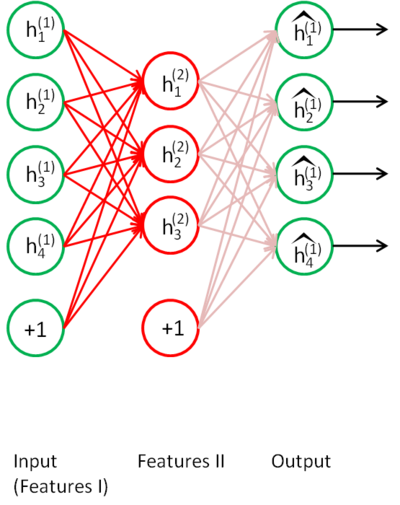
\includegraphics[scale=1]{images/deep_2.png}\\
\caption{The second autoencoder. Then input layer is the hidden layer from the first autoencoder plus a bias unit. While pretraining this autoencoder, the edge weights for all the other layers are frozen. This autoencoder takes the feature output from the first and learns from it, thereby capturing the second-order structure of the data. In general, stacking an extra autoencoder involves using the feature output from the previous as input, adding a hidden and an output layer, and pretrain locally on the same unlabeled data set. The output layer is always removed afterward. \href{http://deeplearning.stanford.edu/wiki/index.php/Stacked_Autoencoders}{\tt Image from UFLDL.}}\label{deep2}
\end{minipage}
\end{figure}




\begin{figure}[H]
\centering
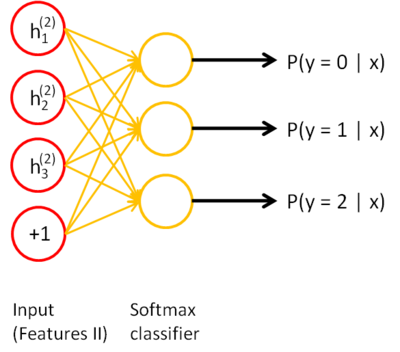
\includegraphics[scale=1.1]{images/deep_3.png}\\
\caption{Pretraining is done for two hidden layers; the final (softmax regressor) 3-classifier is attached.  \href{http://deeplearning.stanford.edu/wiki/index.php/Stacked_Autoencoders}{\tt Image from UFLDL.}}\label{deep3}
% \end{figure}

\hspace{.1\linewidth}

% \begin{figure}[ht]
\centering
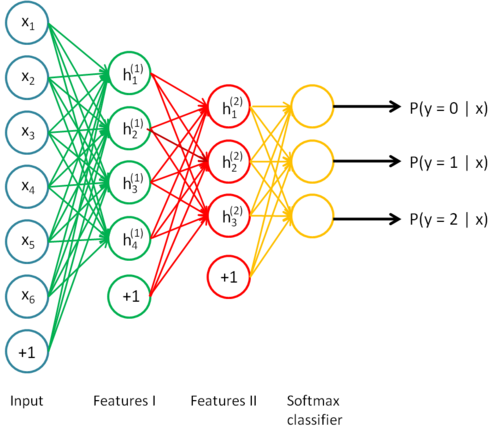
\includegraphics[scale=1.3]{images/deep_4.png}\\
\caption{The resultant deep neural network of 2 hidden layers and a softmax classifier. Fine-tuning can be done on the whole network using backpropagation with gradient descent. The DNN takes in 6 input features $x_1, \cdots, x_6$ to predict the probabilities for 3 possible outcomes $\{0, 1, 2\}$. \href{http://deeplearning.stanford.edu/wiki/index.php/Stacked_Autoencoders}{\tt Image from UFLDL.}}\label{deep4}
\end{figure}


The are two popular yet simple choices of classifiers (ANNs that predict classes of outputs) - \emph{logistic regression} and the \emph{softmax regression} classifiers. The \emph{logistic classifier} is used for outputs that are not mutually exclusive, such as the color and size of a cat. Whereas the \emph{softmax classifier} is for mutually exclusive outputs, such as numerical digits.



\subsection{Variants of Deep Networks}

There are countless variants of deep networks, but their architectures are based off essentially the same ideas - make use of vast amount of data, and adding more hidden layers while still maintaining computational feasibility. They are primarily different in the training techniques, and the propagation of inputs across the network. We give a few of them with quick descriptions.

\begin{enumerate}
	\item {\bf Convolutional Neural Network (ConvNet):} Each layer tends to be arranged into a 2D matrix or pixels, and pooling is done - capturing the statistical properties of a submatrix (a section of the full pixels), such as the max value or the average, and passing it to a pixel on the next layer. This is particularly useful in computer vision, as pooling can capture many local structures such as colors and corners across the layers (such as the example shown in Figure \ref{DNN-fig}).
	\item {\bf Recurrent Neural Network (RNN):} Unlike most neural nets that are feed-forward directed acyclic graphs (DAGs), RNN allows feedback cycles. This allows the output to contribute back to the next inputs, therefore has a strong temporal feature. It's is mostly used for handwriting and speech recognition, in which temporal order plays vital role in making sense of the data.
	\item {\bf Restricted Boltzman Machine (RBM):} This is a feedforward neural net that utilizes special energy function and training algorithm involving Gibbs sampling and Boltzmann distribution. The term ``Restricted'' implies that the hidden and visible layers must form a bipartite graph.
\end{enumerate}






\section{Applications}
It is not an exaggeration to say that machine learning is everywhere today - we are living in the dawn of its golden age. Its rise can be attributed largely to:

\begin{enumerate}
	\item \emph{The invention of efficient algorithms and techniques.} Backpropagation, Self-taught learning, Greedy layer-wise training, and the likes due to Hinton, LeCun and their peers have lifted machine learning out from the theoretical dreamland into the practical world. As a result, many researchers and tech companies rode on the hype and helped propelled the movement further.
	\item \emph{The exponentiation of computational power and the decrease in cost.} Thanks to \emph{Moore's law}, even our smartphones can be a node to train a deep network (as laid in in Google's \emph{TensorFlow} discussed below).
	\item \emph{The abundance of data in the digital age.} This has made obtaining millions or billions of data points possible, and that is precisely why deep network became practical.
	\item \emph{Democratization of the technology.} The popularization of various machine learning APIs and open source libraries such as \emph{IBM Watson, Alchemy, Metamind, Indico, ConvNet, cuDNN, Theano, Torch, TensorFlow} has made using and deploying machine learning close to trivial. They take care of the backend details, allowing for the developers to focus on applying the tools to various problems. Coincidentally, the invention of modern software engineering paradigm helps accelerates the pace of development - today, writing and deploying a full-stack web application while integrating a machine learning module takes just a day, whereas not too long ago it used to take up to weeks.
\end{enumerate}


We next look at the major applications of machine learning throughout modern history.

When Google had its first try at creating artificial intelligence, they did not succeed. However, they did not fail exactly. The product in fact became Google Ad Sense, which powered (and still does) the majority of the company's revenue. This made Google's advertisement recommendation and placement system so advanced that it eclipsed all the other competitors. Given the encouraging outcome, Google would experiment more agressively with A.I. and machine learning in the time to come.

Decades ago linguists have tried to come up with the ultimate algorithm that captures Chomsky's idea of universal grammar - a simple, unifying formal grammar that will capture any human languages. The program had proven most challenging, when even the most respected linguists and computer scientists could not devise an algorithm that could parse and translate between different languages. Despite decades of attempts, we have not come close to realizing Chomsky's original proposition.

Then, Google started its own project, which would then become Google Translate. At that time, Google already had a sufficiently large amount of translated texts, for example between English and French. Instead of devising a collection of production rules and algorithms, the team stuck with an unusual approach - feeding the vast amount of translated texts they had into a neural net. Much to their surprise, it worked, and Google Translate was born. The result was much better than any carefully devised algorithms. No one knew how, but \emph{it worked}. No wonder neural nets are often called a ``black box'', because there is nothing else other than the network and edge weights. If you feed enough data and teaches it about the output, it picks up on the pattern. Neural nets also help Google filter out $99.9\%$ of the spams in Gmail.


2015 is a big year for machine learning - deep networks especially. Google showed off its deep learner that can quickly learn and play games on a super-human level. Google Deep Dream is another publicity stunt, in which an image recognizer spits out new psychedelic images when reversed - it ``dreams'' up images instead of recognizing. IBM Watson got its deep learning upgrade and learned to diagnose diseases and invent new cooking recipe. Facebook released $M$, their A.I. virtual assistant on the \emph{Messenger} app. Weeks after, Google open sourced \emph{TensorFlow}, their machine learning library. We will take a quick look at it.


\subsection{TensorFlow}

Released in November 2015 by Google, \emph{TensorFlow}$^{\ref{tensorflow_paper}}$ is an API library for ``Large-Scale Machine Learning on Heterogeneous Distributed Systems''. Note that this by itself is not a new machine learning technique, but rather a new \emph{architecture} that will streamline how we develop and research with machine learning.

TensorFlow is a culmination of Googlers' experience of deploying machine learning on a large scale. One can see it as a generalized, unified methodology for the commmunity. Generalization gives it flexibility for diverse applications; unification gives all the different team access to a well-maintained, consistent and up-to-date code base. It is already widely used at Google, and has helped many teams work faster and more efficiently.

At first glance, it is a tensor math library (Tensors are simply multidimensional array - scalars are rank-0 tensors, vectors are rank-1, matrices are rank-2, $\cdots$ and so on). It is equipped with many common and performant tensor operators for arithmetic, calculus, transformation, encoding, etc.

There is also many built-in popular machine learning components, such as softmax and logistic regressors, gradient descent and backpropagation algorithms, plain neural nets, and convolutional network with pooling.

\subsubsection{Computation Graph}

The truly novel feature of TensorFlow is its \emph{programming model}. A TensorFlow computation is expressed as a directed graph - we call it the computation graph. A graph node is a computation step, or simply \emph{Op} for \emph{Operation}. This generalizes to the operation of updating state, inputing data and controling the logic. A directed graph edge represents the flow of data encoded in a \emph{tensor}, from the output to the input node. There exists also special edges called \emph{control dependencies} without data-flow - these merely specifies that the \emph{source Op} must complete before the \emph{target Op} can run.

An \emph{Op} has a name such as \emph{multiply, add}, and represents abstract computation. A \emph{kernel} is a device-specific implementation of an operation. Device here refers to physical computation device such as the CPU or GPU. A \emph{Variable} is a special kind of \emph{Op} that allows for tensor-presistence during the runtime.

A \emph{Session} instantiates an empty graph for contruction, and has the \emph{Run} method to run the computation graph once construction is complete.

The data tensors that flow in the directed edges are intuitive to grasp. Tensors are generic and compact for discrete data-encoding; they are also natural to neural networks as we have seen their tensor formalizations before.

The graph-based operation and control flow offer a rich and intuitive programming model. The entire TensorFlow graph can be executed on a single device as usual, but things only get interesting when we consider a distributed execution.

A computation graph can be partitioned into disjoint subgraphs that are then placed on different devices. The overall distributed components, despite being separated, still remember their proper dependencies, thus the entire computation will remain coherent. This resource allocation is also handled automatically in the background. Furthermore, the model is fault-tolerant, as each subgraph can maintain state-persistence or perform independent computation even if some other subgraphs fail. The entire computation can then resume quickly by simply restarting the faulty components, while the healthy ones are always up and ready.

The subgraph-partitioning also allows for partial execution. For a large network, the user can develop and test a subgraph independently by providing special\emph{feed} and \emph{fetch} nodes that simulates data input and output for this subgraph. Such independence makes development easier as one can focus on a more manageable subgraph without having to warry about the larger graph. A subgraph can also be easily replaced by a new module, or be extended, as how one can easily extend a graph by adding edges and nodes.


\subsubsection{Democratization}
Distributed computing with graphs is not by itself anything novel. It is true that TensorFlow is not revolutionary in this sense, but this is not what Google try to do.

The primary contribution of TensorFlow is in \emph{overcoming complexities} - it does not revolutionize machine learning, but it will certainly change \emph{how we do} machine learning.

To illustrate, we show below how easy it is to use TensorFlow to train an ANN with softmax classifier to recognize images of digits.

\begin{lstlisting}[language=Python]

import tensorflow as tf
# import the digit image data
import input_data
mnist = input_data.read_data_sets('MNIST_data', one_hot=True)

# create a new Session, then 
# build the graph below by defining the nodes (Ops)
sess = tf.InteractiveSession()

# the input and output tensors of the ANN, 
# shaped to match the image input dimension (pixels)
x = tf.placeholder("float", shape=[None, 784])
y_ = tf.placeholder("float", shape=[None, 10])

# The weights tensor and the bias tensor
W = tf.Variable(tf.zeros([784,10]))
b = tf.Variable(tf.zeros([10]))

# initialize the Variables
init = tf.initialize_all_variables()

# run the session (graph) to initialize
sess.run(init)

# define the softmax model, also specifying 
# the edges in the graph 
# (e.g. Ops x, W, b and pointing to Op y)
y = tf.nn.softmax(tf.matmul(x,W)+b)
cross_entropy = -tf.reduce_sum(y_*tf.log(y))

# define the training step to use gradient descent
train_step = tf.train.GradientDescentOptimizer(0.01).minimize(cross_entropy)

# run the training on the data, over 1000 iterations
for i in range(1000):
	batch = mnist.train.next_batch(50)
	train_step.run(feed_dict={x: batch[0], y_: batch[1]})
\end{lstlisting}


In less than 20 lines of code, we can train an ANN to recognize images of digits at $98\%$ accuracy - the simplicity achieved with TensorFlow is dramatic. 

Just years ago, practical machine learning was the inaccessible toys of elite academics, mainly due to the implementations being highly technical and complex. Today, any interested person with some understanding of the subject can experiment and build her own machine learners. What TensorFlow has achieved/will achieve is the successful democratization of machine learning.

We look more carefully how TensorFlow democratizes machine learning:

\begin{enumerate}
	\item \emph{The choice of high-level interface language:} Tensorflow is implemented in {\tt C++}, but the language that people interface with it is {\tt Python}, which is a popular and easy-to-use scripting language. This makes everything much easier and concise, as we saw in the example above. More implementations will come soon in other popular languages as well.
	\item \emph{The programming model:} The usage of computation graph is robust and intuitive. The modularity that comes with it also allows users to focus on a much manageable subcomponent of a very large structure.
	\item \emph{Practicality:} The resilient distributed computing and efficient implementation makes the otherwise computation-heavy machine learning practical and fast, as most users can easily use it, and can divide the computation to different devices/resources such as the CPU, GPU of multiple connected machines. Individuals can use it even without owning an entire server farm.
	\item \emph{Scalability:} TensorFlow is built for the individuals as well as the engineering teams at Google. It can be a simple ANN that runs on a laptop, or a gigantic DNN that runs on some dedicated Google server farm. With the distributed computating, it can also run on thousands or millions of devices - like how Google is deploying DNN for Google Translate using the users' smartphones/computers in parts.
	\item \emph{Complexity-handling:} The various features described above - graph construction, dependencies, flow control, device/resource allocation - are all handled automatically in the background. Moreover, many useful \emph{Ops} such as the gradient descend algorithm and the construction of a complete neural net are packaged into built-in functions. What would take hundreds of lines of code if self-implemented now takes only one line in TensorFlow.
	\item \emph{Open source:} The choice to release one of the most powerful proprietary tools of Google to the public isn't unreasonable. With contributions from the community, TensorFlow can improve and grow even faster - it's a win-win situation.
	\item \emph{Bridging the gap:} As part of the needs realized by the research groups at Google, ``It is no longer acceptable to separate research from deployment,'' the company has been trying to shorten the transition between academic research and industrial application. TensorFlow answers the question by providing a unifying platform - researchers can propose and try out new ideas immediately on it, and if they work, send the same source code for the engineer to deploy.
\end{enumerate}


At the time of writing, TensorFlow has only been released for less than a month. The reactions from the community have been welcoming, and people are rapidly picking up and experimenting with the tools. It will be some time before we can see the true impact of TensorFlow - whether or not it will dramatically push machine learning forward.




% In his book \emph{On Intelligence}$^\ref{Hawkins}$, Hawkins 

Hawkins
CLA
Andrew Ng, One learning algorithm






\section{Future Work}






\section{References}


\begin{enumerate}

\item Carnegie Mellon University, \emph{NELL: Never-Ending Language Learning}. \url{http://rtw.ml.cmu.edu/rtw/}\label{NELL}

\item Mitchell, Tom M, \emph{Machine Learning}. New York: McGraw-Hill, 1997.\label{Mitchell}

\item Cybenko., G. \emph{Approximations by superpositions of sigmoidal functions}, Mathematics of Control, Signals, and Systems, 2 (4), 303-314. 1989. \label{Cybenko}

\item Hawkins, Jeff and Blakeslee, Sandra. \emph{On Intelligence.} New York: Henry Holt and, 2005. \label{Hawkins}

\item Ng, Andrew et. al. \emph{UFLDL Tutorial.} \url{http://deeplearning.stanford.edu/wiki/index.php/UFLDL_Tutorial}\label{UFLDL}

\item Dean, Jeffrey et. al. \emph{TensorFlow: Large-Scale Machine Learning on Heterogeneous Distributed Systems}, Google Research. 2015. \label{tensorflow_paper}


\end{enumerate}



\end{document} 

